By assuming the flow through the assembly will be fully isentropic and pseudo one-dimensional it is possible to calculate the state variables at every point knowing the stagnation conditions and the ratio between the cross-sectional area at the point of interest $A_i$ and the at throat of the assembly $A^*$.\\
It must be noted that this is a very radical approximation since for the flow to be  considered pseudo one-dimensional the problem must be reduced to consist purely of variable area ducts.
This clearly overlooks the fact that when entering and leaving the reactor the gas has to perform a right angle turn to follow the flow path.
Another constraint on the duct geometry to achieve reasonable solutions assuming pseudo one-dimensional flow is that the duct must change its cross-sectional area gradually.
\cite{anderson2021modern}
This won't be the case inside the reactor, since there is no way of slicing the reactor chamber to achieve a gradual change in cross-section, especially around the inlet and outlet.
% src/03_analytical-work/1d-flow-geometry.tex

\begin{figure}[H]
	\tikzset{every picture/.style={line width=0.75pt}} %set default line width to 0.75pt        

	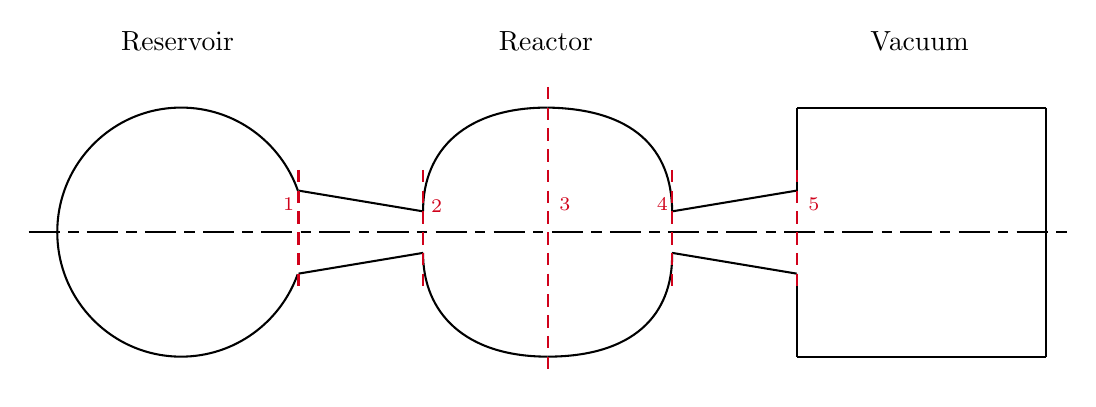
\begin{tikzpicture}[x=0.75pt,y=0.75pt,yscale=-1,xscale=1]
		%uncomment if require: \path (0,300); %set diagram left start at 0, and has height of 300

		%Curve Lines [id:da475214222691565] 
		\draw    (250,130) .. controls (249.86,100.15) and (270.81,79.96) .. (310,80) ;
		%Straight Lines [id:da7887360104686398] 
		\draw    (250,130) -- (190,120) ;
		%Straight Lines [id:da08543915931322243] 
		\draw    (190,160) -- (250,150) ;
		%Curve Lines [id:da8025602502994205] 
		\draw    (250,150) .. controls (249.86,178.82) and (270.15,199.96) .. (310,200) ;
		%Curve Lines [id:da2726691502139771] 
		\draw    (370,130) .. controls (369.86,99.48) and (350.81,80.63) .. (310,80) ;
		%Curve Lines [id:da852756419668889] 
		\draw    (370,150) .. controls (370.53,180.44) and (350.81,199.96) .. (310,200) ;
		%Shape: Arc [id:dp5635876729004141] 
		\draw  [draw opacity=0] (189.58,160.28) .. controls (181.32,183.44) and (159.29,200) .. (133.42,200) .. controls (100.47,200) and (73.76,173.14) .. (73.76,140) .. controls (73.76,106.86) and (100.47,80) .. (133.42,80) .. controls (159.41,80) and (181.52,96.71) .. (189.7,120.04) -- (133.42,140) -- cycle ;

		\draw   (189.58,160.28) .. controls (181.32,183.44) and (159.29,200) .. (133.42,200) .. controls (100.47,200) and (73.76,173.14) .. (73.76,140) .. controls (73.76,106.86) and (100.47,80) .. (133.42,80) .. controls (159.41,80) and (181.52,96.71) .. (189.7,120.04) ;  

		%Straight Lines [id:da851456234203132] 
		\draw    (430,120) -- (395.21,125.8) -- (370,130) ;

		%Straight Lines [id:da4472765006336461] 
		\draw    (430,160) -- (370,150) ;

		%Straight Lines [id:da002945503090612256] 
		\draw    (430,160) -- (430,200) ;

		%Straight Lines [id:da8471350272235534] 
		\draw    (430,200) -- (550,200) ;

		%Straight Lines [id:da5527680318892192] 
		\draw    (430,120) -- (430,80) ;

		%Straight Lines [id:da07985332663257294] 
		\draw    (550,80) -- (430,80) ;

		%Straight Lines [id:da34251808578753806] 
		\draw [line width=0.75]  [dash pattern={on 11.25pt off 3pt on 3.75pt off 3pt}]  (60,140) -- (560,140) ;

		%Straight Lines [id:da9033197197458074] 
		\draw [color={rgb, 255:red, 208; green, 2; blue, 27 }  ,draw opacity=1 ] [dash pattern={on 4.5pt off 3pt}]  (190,110) -- (190,170) ;

		%Straight Lines [id:da3235152821308156] 
		\draw [color={rgb, 255:red, 208; green, 2; blue, 27 }  ,draw opacity=1 ] [dash pattern={on 4.5pt off 3pt}]  (250,110) -- (250,170) ;

		%Straight Lines [id:da6817412504038962] 
		\draw [color={rgb, 255:red, 208; green, 2; blue, 27 }  ,draw opacity=1 ] [dash pattern={on 4.5pt off 3pt}]  (370,110) -- (370,170) ;

		%Straight Lines [id:da4311097348294681] 
		\draw [color={rgb, 255:red, 208; green, 2; blue, 27 }  ,draw opacity=1 ] [dash pattern={on 4.5pt off 3pt}]  (310,70) -- (310,210) ;

		%Straight Lines [id:da3223431791972775] 
		\draw [color={rgb, 255:red, 208; green, 2; blue, 27 }  ,draw opacity=1 ] [dash pattern={on 4.5pt off 3pt}]  (430,110) -- (430,170) ;

		%Straight Lines [id:da8828390660283978] 
		\draw    (550,80) -- (550,200) ;

		% Text Node
		\draw (103,42) node [anchor=north west][inner sep=0.75pt]   [align=left] {Reservoir};

		% Text Node
		\draw (285,42) node [anchor=north west][inner sep=0.75pt]   [align=left] {Reactor};

		% Text Node
		\draw (464,42) node [anchor=north west][inner sep=0.75pt]   [align=left] {Vacuum};

		% Text Node
		\draw (178,122) node [anchor=north west][inner sep=0.75pt]  [font=\scriptsize,color={rgb, 255:red, 208; green, 2; blue, 27 }  ,opacity=1 ] [align=left] {\begin{minipage}[lt]{8.67pt}\setlength\topsep{0pt}
		\begin{center}
		1
		\end{center}

		\end{minipage}};
		% Text Node
		\draw (256.5,127.5) node  [font=\scriptsize,color={rgb, 255:red, 208; green, 2; blue, 27 }  ,opacity=1 ] [align=left] {\begin{minipage}[lt]{8.67pt}\setlength\topsep{0pt}
		\begin{center}
		2
		\end{center}

		\end{minipage}};
		% Text Node
		\draw (311,122) node [anchor=north west][inner sep=0.75pt]  [font=\scriptsize,color={rgb, 255:red, 208; green, 2; blue, 27 }  ,opacity=1 ] [align=left] {\begin{minipage}[lt]{8.67pt}\setlength\topsep{0pt}
		\begin{center}
		3
		\end{center}

		\end{minipage}};
		% Text Node
		\draw (358,122) node [anchor=north west][inner sep=0.75pt]  [font=\scriptsize,color={rgb, 255:red, 208; green, 2; blue, 27 }  ,opacity=1 ] [align=left] {\begin{minipage}[lt]{8.67pt}\setlength\topsep{0pt}
		\begin{center}
		4
		\end{center}

		\end{minipage}};
		% Text Node
		\draw (431,122) node [anchor=north west][inner sep=0.75pt]  [font=\scriptsize,color={rgb, 255:red, 208; green, 2; blue, 27 }  ,opacity=1 ] [align=left] {\begin{minipage}[lt]{8.67pt}\setlength\topsep{0pt}
		\begin{center}
		5
		\end{center}

		\end{minipage}};
	\end{tikzpicture}
\caption{Mean velocity parallel to the flow at a point $x$ inside a constant area duct in molecular flow.}
\label{fig:1D-flow-geometry}
\end{figure}

\cite{SALAS1986193}
\cite{EMMONS1958}
